\documentclass{article}
\usepackage[utf8]{inputenc}
\usepackage{amsmath}
\usepackage{graphicx}
\usepackage{hyperref}
\usepackage{tikz}
\usepackage{float}
\usepackage{verbatim}
\usetikzlibrary{automata,positioning}


\title{PDF Lexical Analysis}
\author{Boujamaa ATRMOUH}
\date{\today}

\begin{document}

\maketitle

\section{Introduction}

\begin{flushleft}
    \hspace{1cm}The objective of this project is to develop a series of tools that, given a PDF file, can extract information about its structure. To do this, we will develop different parsers with the aim of analyzing the content of a file. Ideally, these tools should be able to serve as a basis for the development of code that can repair, or even edit, a PDF file.
\end{flushleft}

\section{PDF Structure}


\begin{flushleft}
    \hspace{1cm}Addressing all the subtleties of the PDF format would be far too ambitious, and we will therefore make the following assumptions about the argument file:
    \begin{itemize}
        \item The document is not protected by encryption;
        \item The file contains only one reference table;
        \item This reference table is not compressed;
        \item PDF objects are defined directly in the body of the document (and not within a stream);
        \item Streams never contain the sequence of characters "endstream". This string will therefore always represent the end of stream marker;
        \item Parentheses within PDF character strings are always preceded by the character.
    \end{itemize}
In practice, this means that our code will be able to handle almost all PDF files in version 1.4 (or lower), unencrypted and without incremental modification.
\end{flushleft}

\subsection*{I}

\begin{flushleft}
    \hspace{1cm} Files \texttt{parser1.y} and \texttt{lexer1.l}.
The main program takes as its only argument the path to the file to be analyzed. If this file is not valid, an error message will be displayed. If it is valid, the version of the PDF format and the address of the reference table will be displayed on the standard output.

\begin{itemize}
    \item \texttt{VERSION} is a lexeme to represent comments of the form \%PDF-x,y,
    \item \texttt{LINE} is a lexeme to represent any other line of the file,
    \item \texttt{lines} is a non-terminal symbol, representing a sequence of lines from which the last line must be extracted, verify that it contains only a positive integer, and display this integer.
\end{itemize}

\end{flushleft}

\begin{figure}[H]
    \centering
    \scalebox{.8}{
    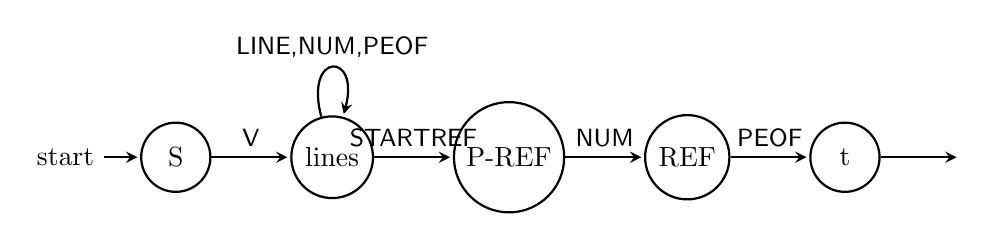
\begin{tikzpicture}[->,>=stealth,shorten >=1pt,auto,node distance=1cm,
        thick,main node/.style={circle,draw,font=\sffamily\Large\bfseries}]
    
    \node[state, initial] (S) {S};
    \node[state] (lines) [right=of S] {lines};
    \node[state] (P-REF) [right=of lines] {P-REF};
    \node[state] (REF) [right=of P-REF] {REF};
    \node[state] (t) [right=of REF] {t};
    
    \node[draw=none, right=of t] (dummy) {};
    
    \path[every node/.style={font=\sffamily\small}]
    (S) edge node {V} (lines)
    (lines) edge [loop above] node {LINE,NUM,PEOF} (lines)
    (lines) edge node {STARTREF} (P-REF)
    (P-REF) edge node {NUM} (REF)
    (REF) edge node {PEOF} (t)
    (t) edge [->] (dummy);
    \end{tikzpicture}
    }
    \caption{automata I}
\end{figure}

\begin{figure}[H]
    \centering
    \begin{minipage}[t]{0.45\linewidth}
        \centering
        \[
        S \rightarrow \text{VERSION} \; \text{lines} \; \text{PEOF}
        \]
        \[
        \text{lines} \rightarrow \text{STARTREF} \; \text{NUM} 
        \]
        \[
        \mid \text{LINE} \; \text{lines}
        \]
        \[
            \mid \text{NUM} \; \text{lines} 
        \]
        \[
        \mid \text{PEOF} \; \text{lines}
        \]
        \caption{I: Grammar}
    \end{minipage}
\hfill
\begin{minipage}[t]{0.45\linewidth}
    \centering
    \[
    S \rightarrow \text{VERSION} \; \text{lines}
    \]
    \[
    \text{lines} \rightarrow \text{LINE} \; \text{lines}
    \]
    \[
    \mid \text{NUM} \; \text{lines}
    \]
    \[
    \mid \text{PEOF} \; \text{lines}
    \]
    \[
    \mid \text{STARTREF} \; \text{ref}
    \]
    \[
    \text{ref} \rightarrow \text{NUM} \; \text{end\_line}
    \]
    \[
    \text{end\_line} \rightarrow \text{PEOF}
    \]
    \caption{I: Right-linear grammar}
\end{minipage}
\end{figure}

\[\text{VERSION} = \verb|%PDF-[0-9]+\.[0-9]+|\]
\[\text{LINE} = \verb|[^\n]+|\]
\[\text{NUM} = \verb|[0-9]+|\]
\[\text{PEOF} = \verb|%%EOF|\]
\[\text{STARTREF} = \verb|startxref|\]

\begin{tabular}{|l|p{10cm}|}
    \hline
    \textbf{Command} & \textbf{Description} \\
    \hline
    \texttt{make} & Compile the parser and lexer. \\
    \hline
    \texttt{make debug} & Compile in debug mode. \\
    \hline
    \texttt{make test} & Generate PDF files and test them. \\
    \hline
    \texttt{make testsNoLog} & Similar to \texttt{make test}, but with a clean console output. \\
    \hline
\end{tabular}

\subsection*{II}

Once the reference table address is known, further analysis of the end of a PDF file becomes possible. This involves validating a reference table and a trailer, which are essential components of a PDF file structure.

\subsubsection*{Reference Table Structure}

A valid reference table in a PDF file consists of the following elements:

\begin{enumerate}
    \item \textbf{Header Line (\texttt{xref})}: Indicates the beginning of the reference table.
    
    \item \textbf{Table Entries}: Each entry in the table provides information about a PDF object. The structure of each entry includes:
    \begin{itemize}
        \item Object Address: A 10-digit address.
        \item Generation Number: A 5-digit number indicating the generation of the object.
        \item Type: Either 'n' (normal) or 'f' (free).
    \end{itemize}
    
    These entries are typically organized in a format similar to:
    \begin{verbatim}
    0000000015 00002 n
    0000000025 00000 n
    \end{verbatim}
    
    Here, \texttt{0000000015} is the object address, \texttt{00002} is the generation number, and \texttt{n} indicates it's a normal object.
    
    \begin{figure}[H]
        \centering
        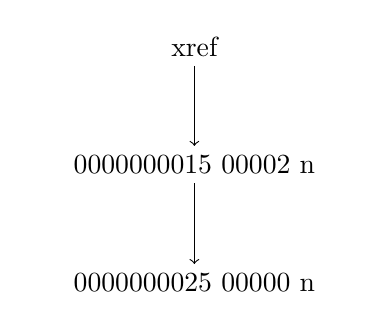
\begin{tikzpicture}[node distance=1.5cm, auto]
            \node (header) [text width=4cm, align=center] {xref};
            \node (entry1) [below of=header, text width=4cm, align=center] {0000000015 00002 n};
            \node (entry2) [below of=entry1, text width=4cm, align=center] {0000000025 00000 n};
            
            \draw[->] (header) -- (entry1);
            \draw[->] (entry1) -- (entry2);
        \end{tikzpicture}
        \caption{Schematic Representation of a Reference Table}
        \label{fig:reference_table}
    \end{figure}
    
\end{enumerate}

\subsubsection*{Trailer Structure}

After the reference table, a valid PDF file trailer includes:

\begin{enumerate}
    \item \textbf{Trailer Keyword}: Marks the start of the trailer section.
    
    \item \textbf{Dictionary}: A structured set of key-value pairs enclosed between \texttt{<<} and \texttt{>>}.
    
    \item \textbf{Startxref}: Indicates the position of the start of the cross-reference table.
    
    \item \textbf{Cross-reference Table Start Address}: An integer pointing to the beginning of the reference table.
    
    \item \textbf{End-of-File Marker (\texttt{\%\%EOF})}: Special comment indicating the end of the PDF file.
    
    \begin{figure}[H]
        \centering
        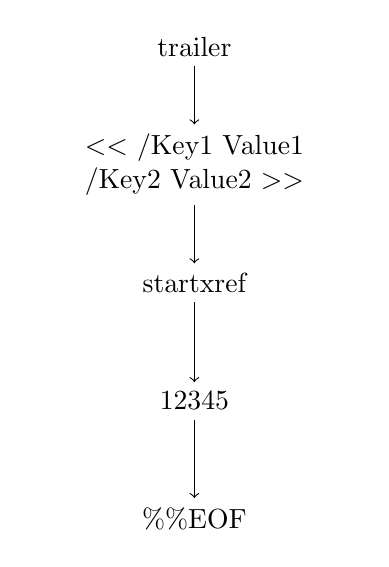
\begin{tikzpicture}[node distance=1.5cm, auto]
            \node (trailer) [text width=4cm, align=center] {trailer};
            \node (dict) [below of=trailer, text width=4cm, align=center] {$<<$ /Key1 Value1 /Key2 Value2 $>>$};
            \node (startxref) [below of=dict, text width=4cm, align=center] {startxref};
            \node (address) [below of=startxref, text width=4cm, align=center] {12345};
            \node (eof) [below of=address, text width=4cm, align=center] {\%\%EOF};
            
            \draw[->] (trailer) -- (dict);
            \draw[->] (dict) -- (startxref);
            \draw[->] (startxref) -- (address);
            \draw[->] (address) -- (eof);
        \end{tikzpicture}
        \caption{Schematic Representation of a PDF Trailer}
        \label{fig:pdf_trailer}
    \end{figure}
    
\end{enumerate}
    
 Data Structures: A \texttt{PDFObject} structure is defined to store information about PDF objects, including their address, object ID, and generation number. This structure is managed through functions like \texttt{createPDFObject}, \texttt{insertPDFObject}, \texttt{printPDFObjects}, and \texttt{freePDFObjects}.

\begin{tabular}{|l|p{10cm}|}
    \hline
    \textbf{Command} & \textbf{Description} \\
    \hline
    \texttt{make} & Compile the parser and lexer. \\
    \hline
    \texttt{make debug} & Compile in debug mode. \\
    \hline
    \texttt{make testSingle} & Run a single test. \\
    \hline
\end{tabular}

\newpage

\subsection*{III}

The objective of this section is to develop a parser for valid PDF objects. According to the PDF specification, a valid PDF object can take several forms, each with specific characteristics that must be recognized and validated.

To parse and recognize different types of PDF objects, we define a grammar and corresponding lexical rules using \texttt{parser3.y} and \texttt{lexer3.l}. These files work together to identify and classify PDF objects based on their format and content.

In \texttt{lexer3.l}, lexical rules are defined using regular expressions to match various types of PDF objects:
\begin{itemize}
    \item \textbf{Null, Boolean, Integer, Real}: Identified using specific patterns (\texttt{null}, \texttt{boolean}, \texttt{signedInt}, \texttt{signedReal}).
    \item \textbf{Strings}: Regular and hexadecimal strings enclosed in parentheses (\texttt{string}, \texttt{hexString}).
    \item \textbf{Names}: Start with \texttt{/} and can include any character except whitespace and specific delimiters (\texttt{name}).
    \item \textbf{References}: Composed of two integers followed by \texttt{R} (\texttt{ref}).
    \item \textbf{Lists}: Enclosed in square brackets (\texttt{startList}, \texttt{endList}).
    \item \textbf{Dictionaries}: Enclosed in double angle brackets (\texttt{startDict}, \texttt{endDict}).
\end{itemize}

The grammar in \texttt{parser3.y} specifies how these tokens are structured to form valid PDF objects:

\begin{tabular}{|l|p{10cm}|}
    \hline
    \textbf{Command} & \textbf{Description} \\
    \hline
    \texttt{make} & Compile the parser and lexer. \\
    \hline
    \texttt{make debug} & Compile in debug mode. \\
    \hline
\end{tabular}


\end{document}